\documentclass[12pt,letterpaper]{article}
\usepackage[utf8]{inputenc}
\usepackage[spanish]{babel}
\usepackage{graphicx}
\usepackage[left=2cm,right=2cm,top=2cm,bottom=2cm]{geometry}
\usepackage{graphicx} % figuras
% \usepackage{subfigure} % subfiguras
\usepackage{float} % para usar [H]
\usepackage{amsmath}
%\usepackage{txfonts}
\usepackage{stackrel} 
\usepackage{multirow}
\usepackage{enumerate} % enumerados
\renewcommand{\labelitemi}{$-$}
\renewcommand{\labelitemii}{$\cdot$}


% \author{}
% \title{Caratula}
\begin{document}

% Fancy Header and Footer
% \usepackage{fancyhdr}
% \pagestyle{fancy}
% \cfoot{}
% \rfoot{\thepage}
%

% \usepackage[hidelinks]{hyperref} % CREA HYPERVINCULOS EN INDICE

% \author{}
\title{Caratula}

\begin{titlepage}
\begin{center}
\large{UNIVERSIDAD PRIVADA DE TACNA}\\
\vspace*{-0.025in}
\begin{figure}[htb]
\begin{center}

\includegraphics[width=8cm]{./Imagenes/logo}
\end{center}
\end{figure}
\vspace*{0.15in}
INGENIERIA DE SISTEMAS  \\

\vspace*{0.5in}
\begin{large}
TITULO:\\
\end{large}

\vspace*{0.1in}
\begin{Large}
\textbf{Informe 05 Configuracion Base de datos Oracle} \\
\end{Large}

\vspace*{0.3in}
\begin{Large}
\textbf{CURSO:} \\
\end{Large}

\vspace*{0.1in}
\begin{large}
BASE DE DATOS II\\
\end{large}

\vspace*{0.3in}
\begin{Large}
\textbf{DOCENTE(ING):} \\
\end{Large}

\vspace*{0.1in}
\begin{large}
 Patrick Cuadros Quiroga\\
\end{large}

\vspace*{0.2in}
\vspace*{0.1in}
\begin{large}
Alumno: \\
\begin{flushleft}
Jhosmell Gyno Alfaro Musaja\hfill	(201505323) \\
Katerin Almendra Merino Quispe\hfill 	(2018060918) \\
Nilton Edy Perez Mamani\hfill 	(2015053233) \\
Jhon Peter Aguilar Atencio\hfill 	(2015053222) \\
\end{flushleft}
\end{large}
\end{center}

\end{titlepage}


\tableofcontents % INDICE
\thispagestyle{empty} % INDICE SIN NUMERO
\newpage
\setcounter{page}{1} % REINICIAR CONTADOR DE PAGINAS DESPUES DEL INDICE


\begin{Large}
\begin{center}
\textbf{Contenido} \\
\end{center}
\end{Large}

\section{Contenido} 


\begin{itemize}
	\begin{center}
	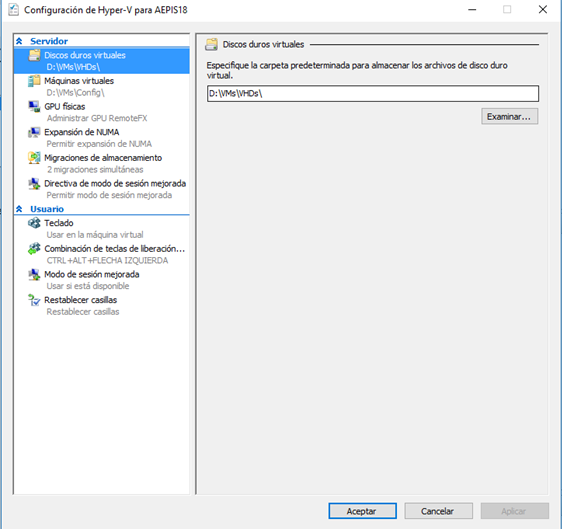
\includegraphics[width=14cm]{./Imagenes/imagen2} 
	\end{center}

	\item En definitiva utilizar una u otra depende de tus n.



\end{itemize} 
\begin{itemize}
	\begin{center}
	    Paso 1
	\end{center}
	

	    Primero abrimos el Hyper-v, nos dirijimos donde dice Administrador de conmutadores virtuales hacemos click, después se abrirá otra ventana donde saldrá para crear el Conmmutador Virtual le colocamos cualquier nombre, como lo puedes observar en la siguiente imagen.
		\begin{center}
		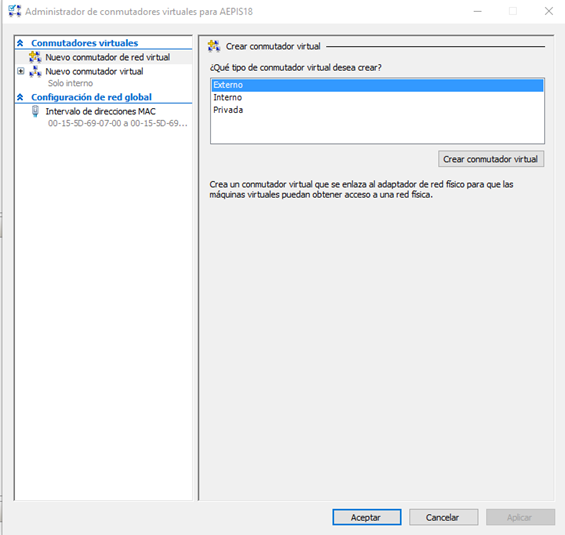
\includegraphics[width=15cm]{./Imagenes/imagen1} 
		\end{center}
	

	\end{itemize} 
	

	\begin{itemize}
	\begin{center}
	    Paso 2
	\end{center}
	

	    Despues nos dirigimos a Configuracion de hyper-v, se abrirá una ventana. 
		\begin{center}
		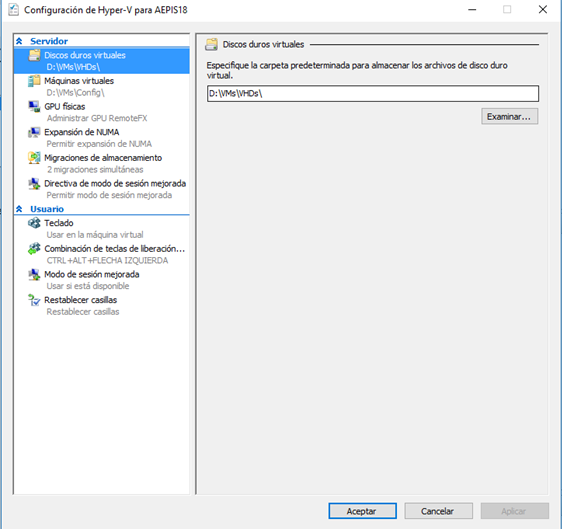
\includegraphics[width=15cm]{./Imagenes/imagen2} 
		\end{center}
	

	\end{itemize} 
	
	
	\begin{itemize}
	\begin{center}
  	  Paso 3
	\end{center}


   	 Seguidamente hacemos click en Discos Duros Virtuales\\
	\begin{center}
	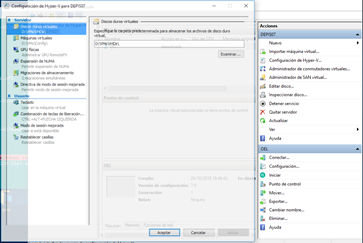
\includegraphics[width=15cm]{./Imagenes/imagen3} 
	\end{center}


	\end{itemize} 


	\begin{itemize}
	\begin{center}
 	   Paso 4
	\end{center}


   	 Luego hacemos click en examinar y agregamos la siguiente carpeta que creamos en el Disco D, con el nombre de VHDs, le damos click en Seleccionar Carpeta, como se puede observar en la imagen.\\
	\begin{center}
	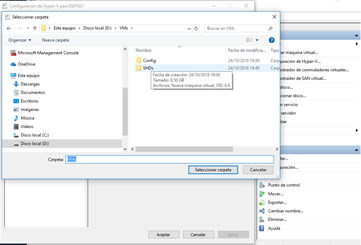
\includegraphics[width=15cm]{./Imagenes/imagen4} 
	\end{center}


	\end{itemize}
	
	\begin{itemize}
	\begin{center}
    Paso 5
	\end{center}


   Despues seleccionamos Maquinas Virtuales y le hacemos click en examinar.\\
	\begin{center}
	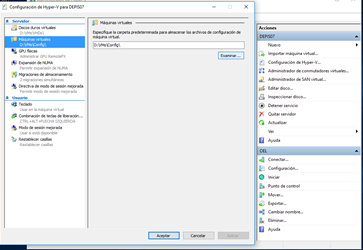
\includegraphics[width=15cm]{./Imagenes/imagen5} 
	\end{center}


	\end{itemize} 


	\begin{itemize}
	\begin{center}
   	 Paso 6
	\end{center}


 	   Continuando con el paso anterior se abrirá una ventana donde seleccionamos la siguiente carpeta con el nombre de Config, le hacemos click en Selecciona Carpeta. Despues le damos click en Aplicar y después en aceptar. \\
	\begin{center}
	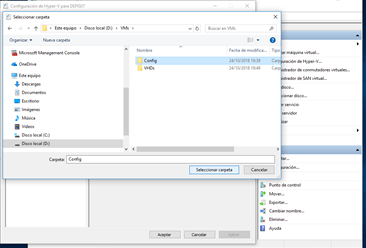
\includegraphics[width=15cm]{./Imagenes/imagen6} 
	\end{center}


	\end{itemize} 


  
  
  


\documentclass{article}
\usepackage[utf8]{inputenc}

\title{Pagina03}

\begin{document}

\section{Paso 15:} 
\begin{itemize}
	\item Ahora seguiremos con la instalacion dejaremos que instale para luego poder logearnos con nuestro codigo.
	\begin{center}
	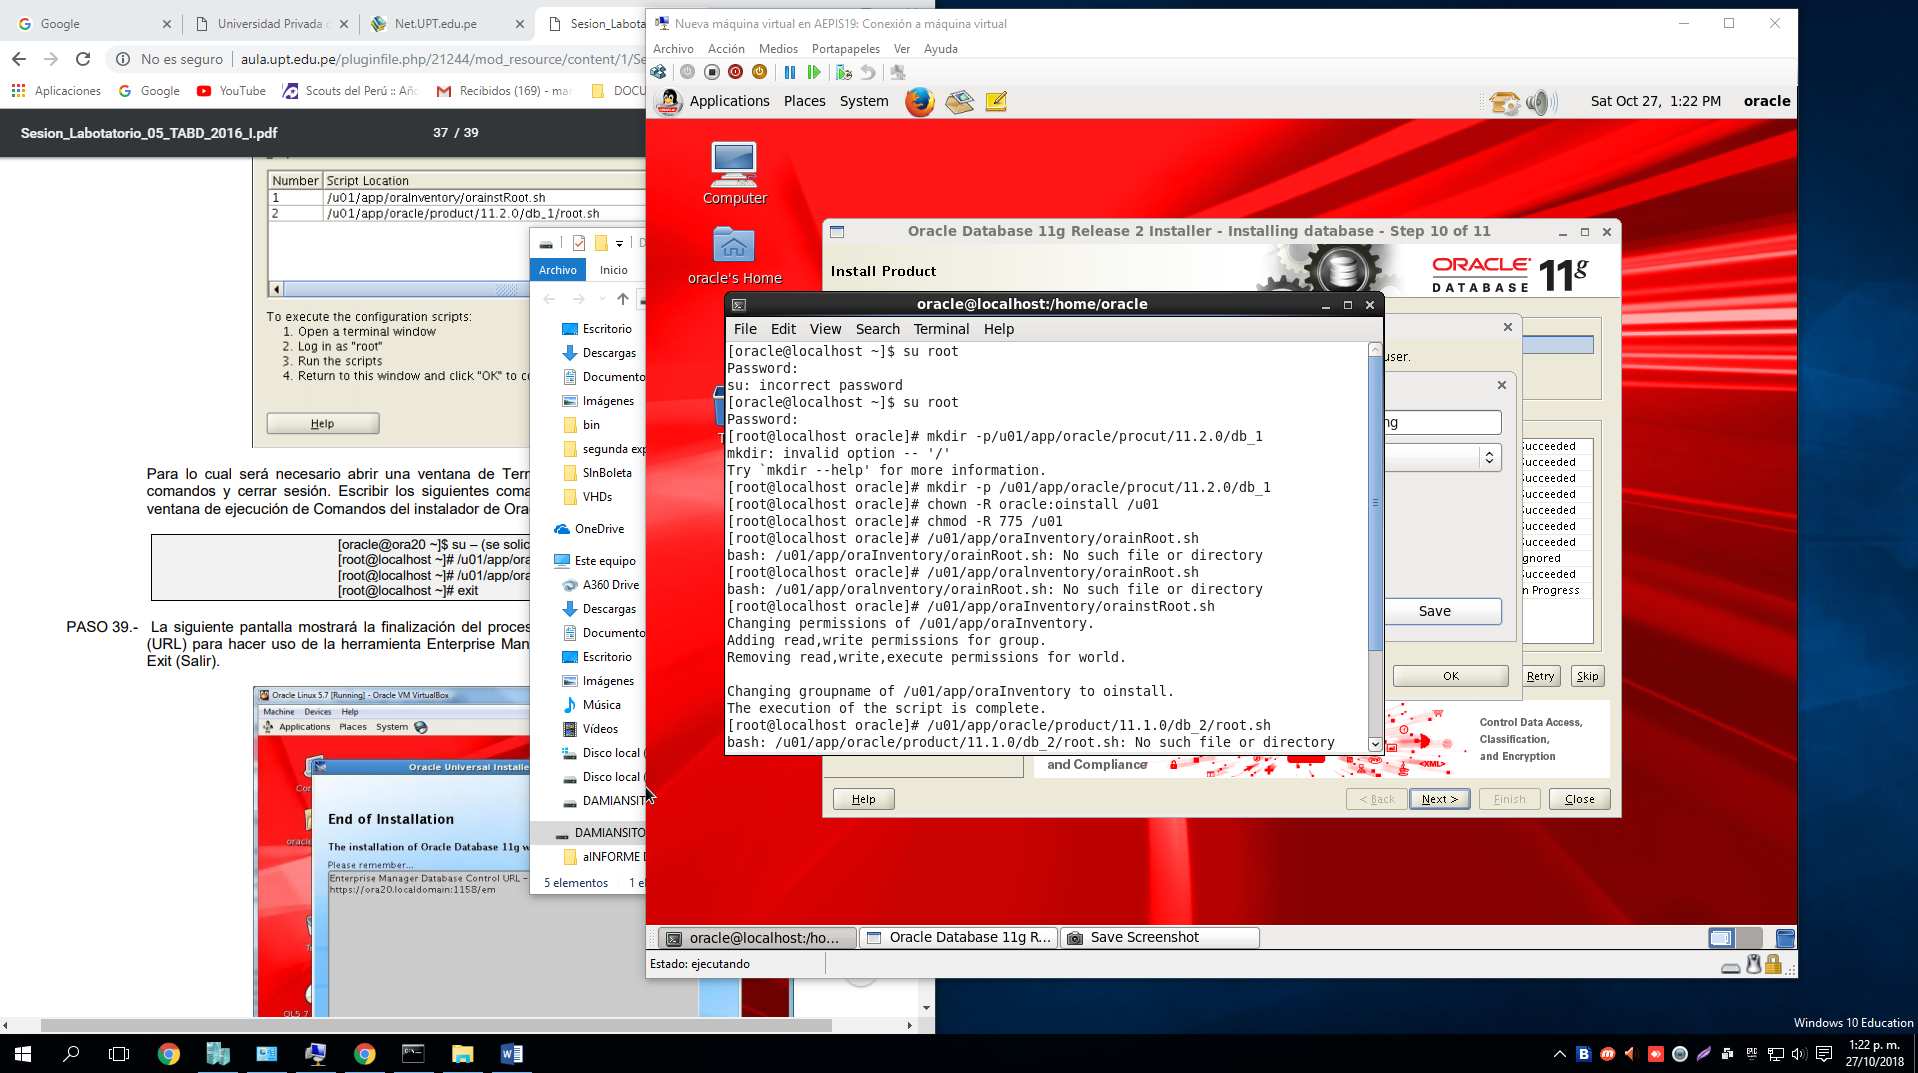
\includegraphics[width=14cm]{./Imagenes/imagen15} 
	\end{center}
	
\section{Paso 16:}
	\item Ahora seguidamente damos siguiente hasta llegar a este punto de finish, para luego dar close y termina la instalacion.
	\begin{center}
	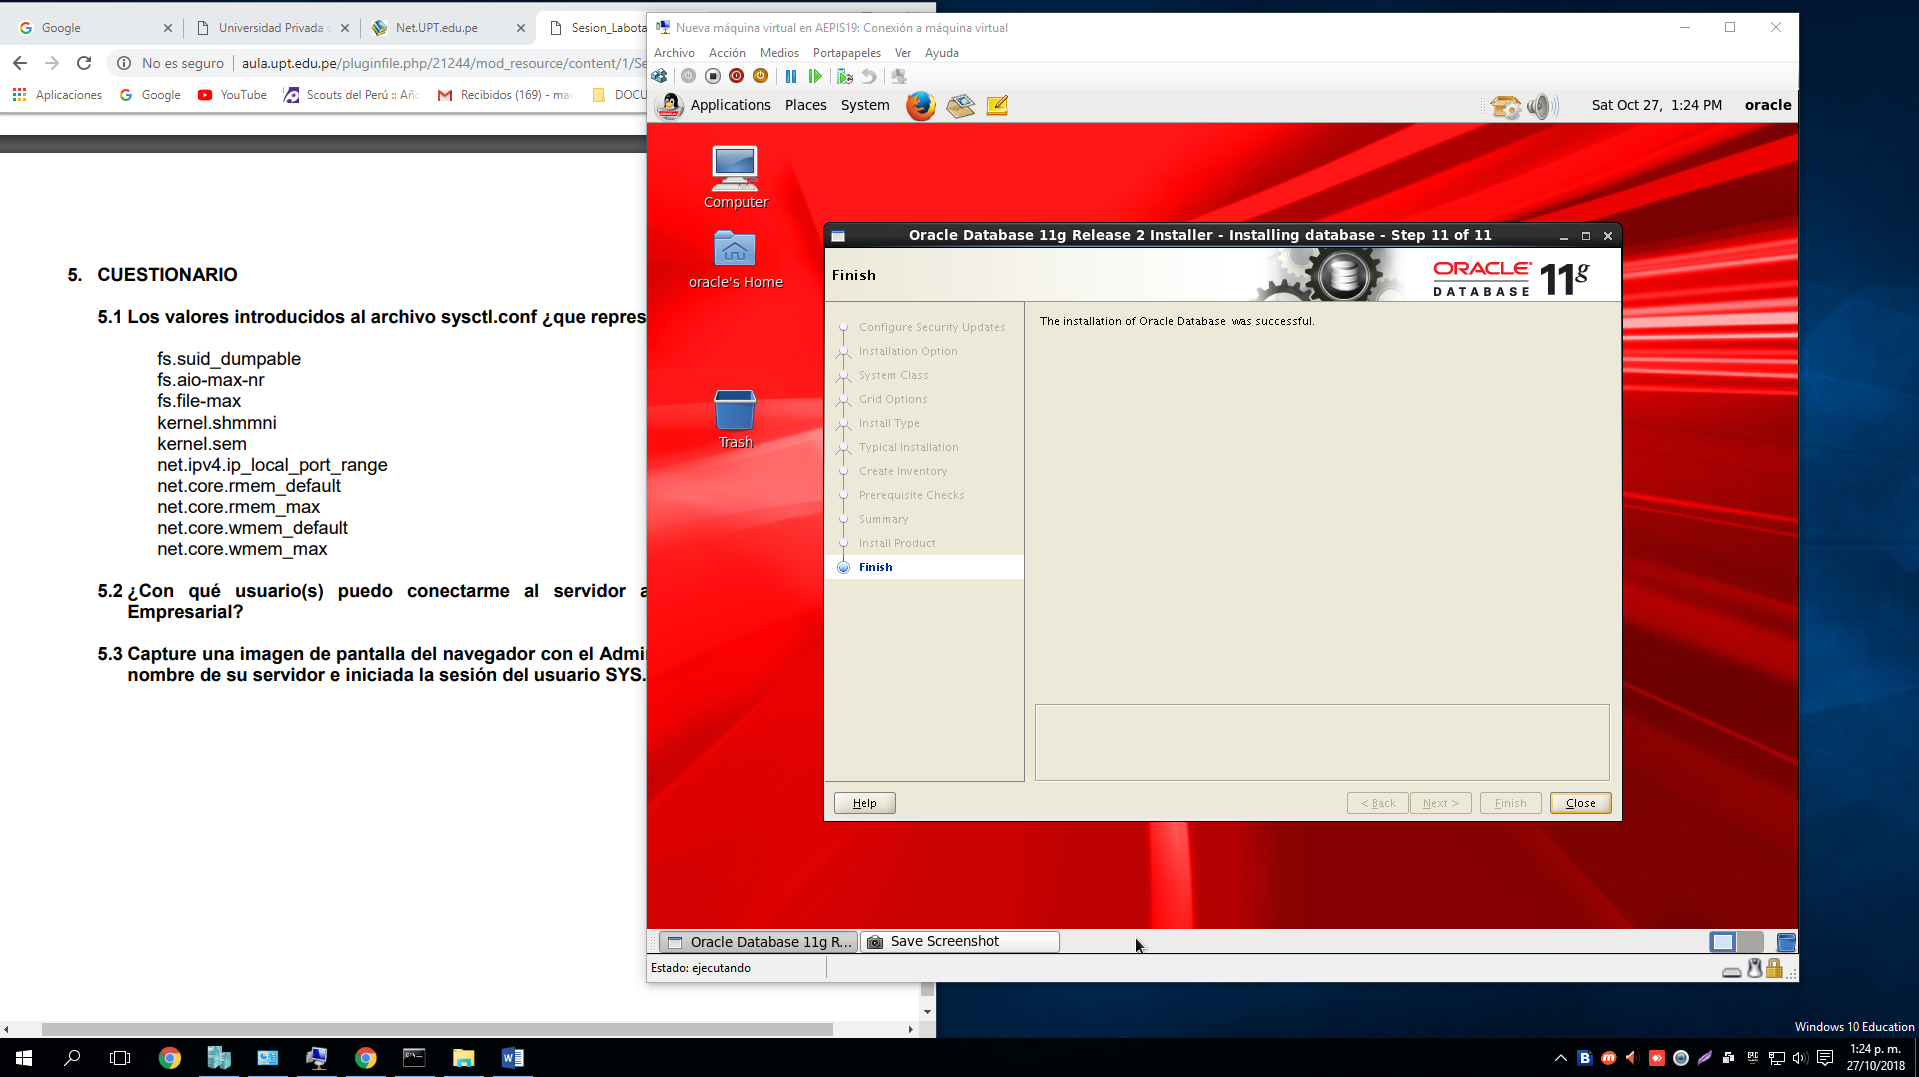
\includegraphics[width=14cm]{./Imagenes/imagen16} 
	\end{center}
\newpage
\section{Paso 17:} 
	\item Ahora reiniciamos la maquina virtual, mirando el ping de la maquina virtal, para su uso correcto.
	\begin{center}
	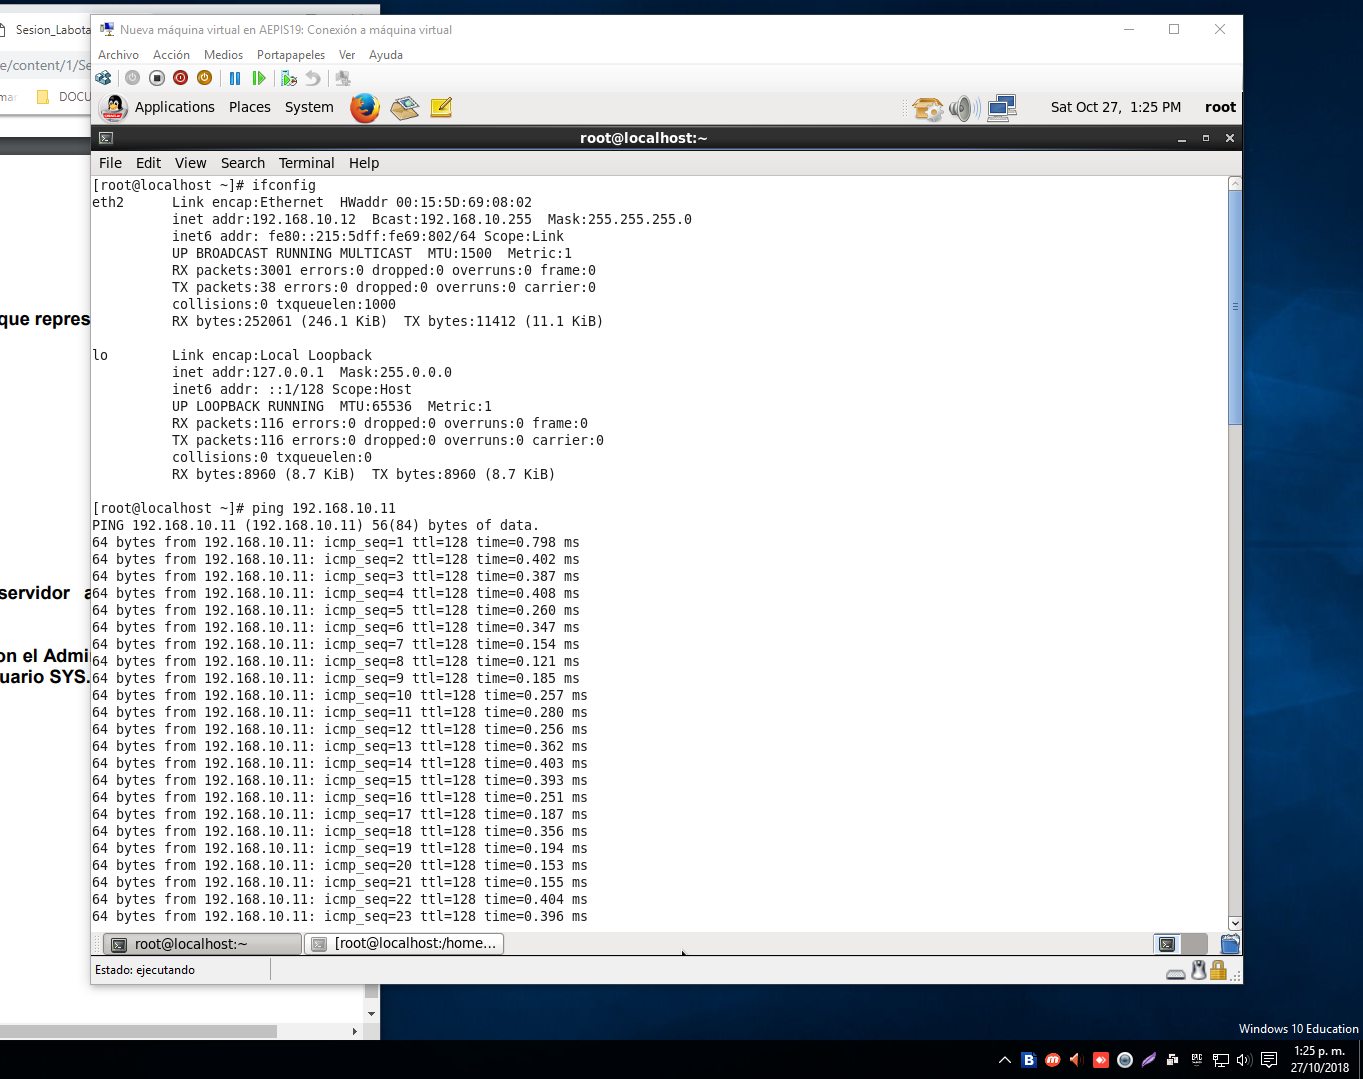
\includegraphics[width=14cm]{./Imagenes/imagen17} 
	\end{center}
\section{Paso 18:} 
	\item Seguidamente buscamos el cd de oracle para que el funionamiento esa correcto.
	\begin{center}
	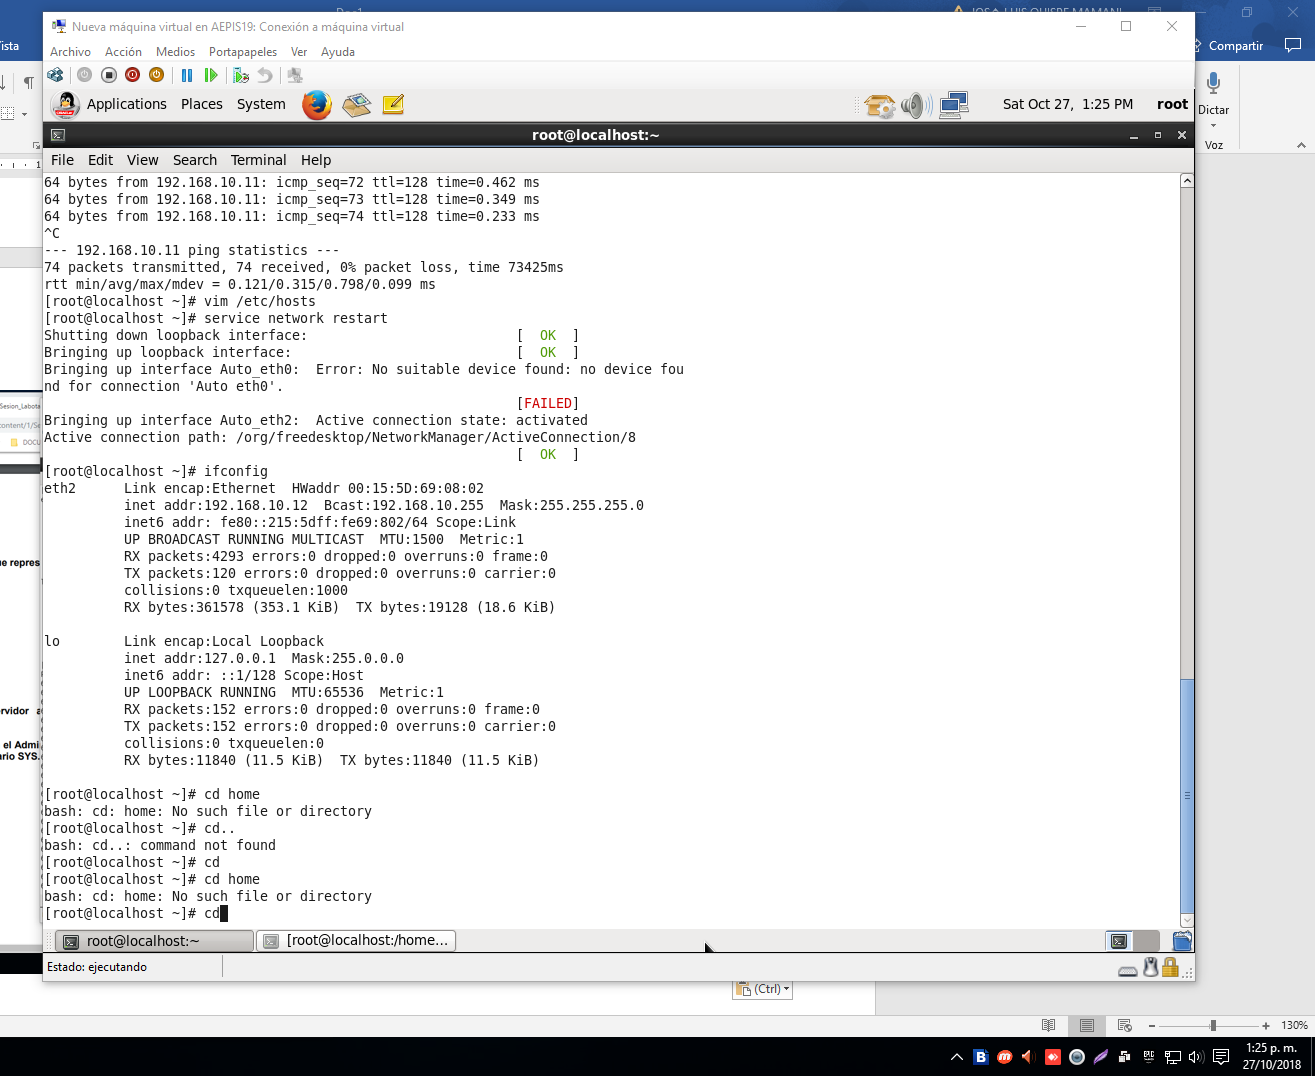
\includegraphics[width=14cm]{./Imagenes/imagen18} 
	\end{center}
\newpage
\section{Paso 19:} 
	\item Continuamos con la instalacion la parte del cd oracle.
	\begin{center}
	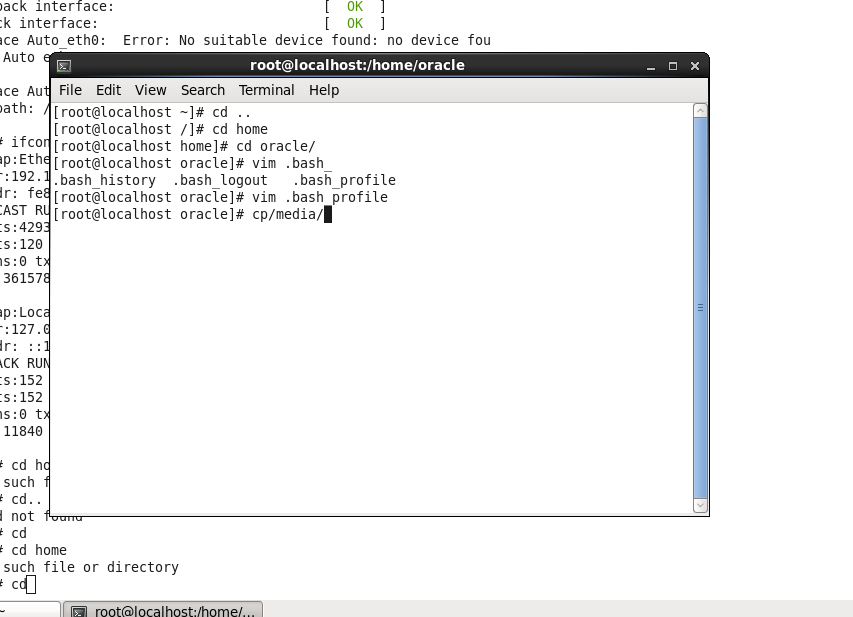
\includegraphics[width=13cm]{./Imagenes/imagen19} 
	\end{center}

\section{Paso 20:}
	\item continuando con la instalacion del Oracle.
	\begin{center}
	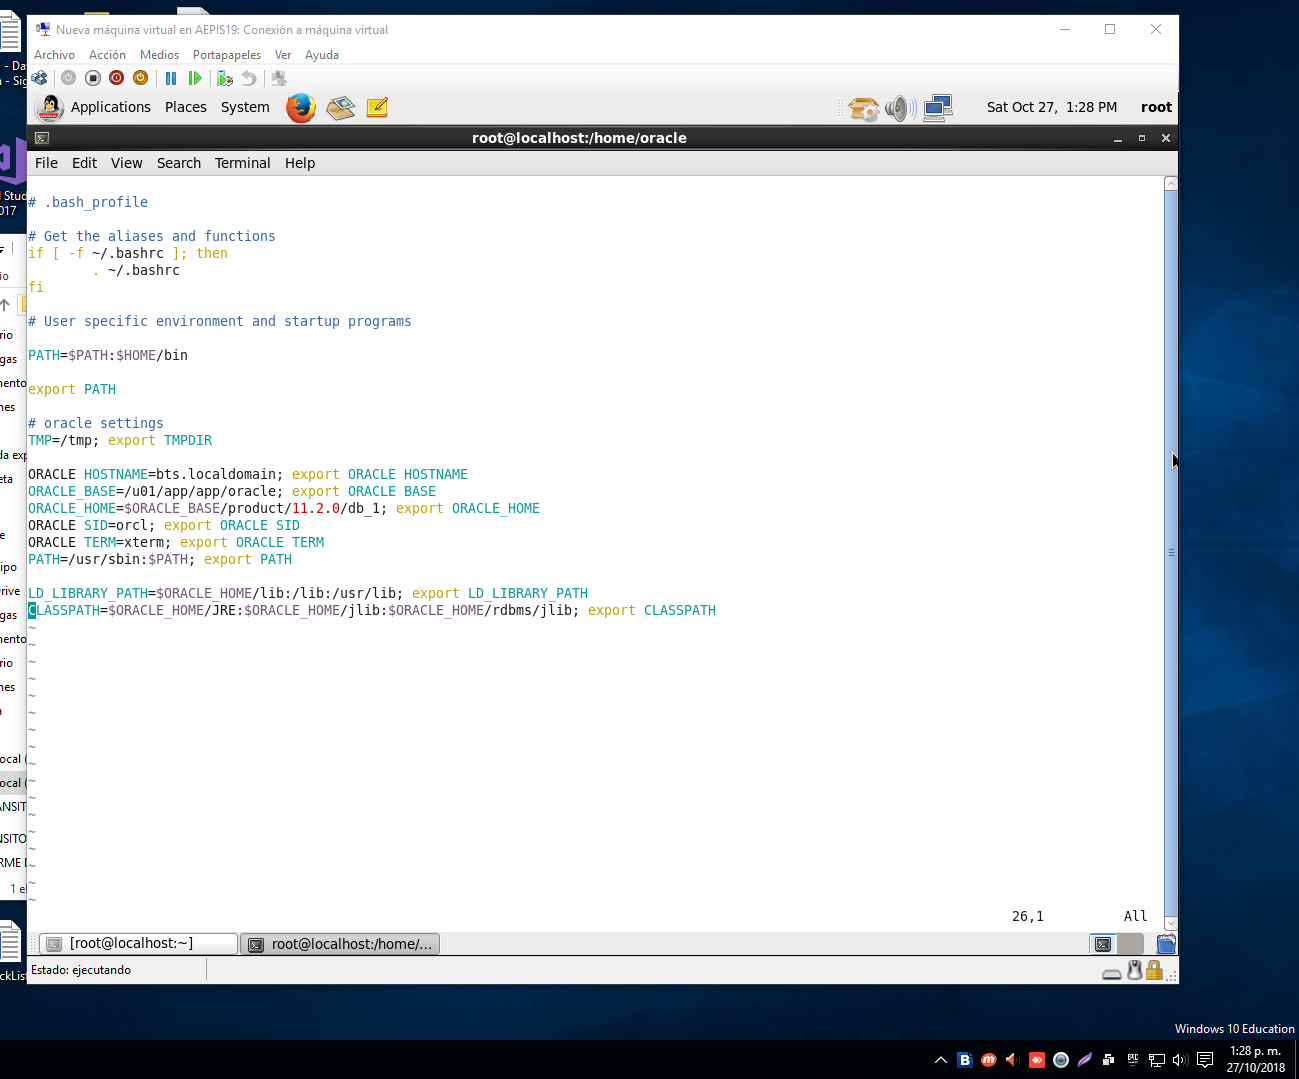
\includegraphics[width=13cm]{./Imagenes/imagen20} 
	\end{center}
	
\newpage
\section{Paso 21:}
	\item continuando con la instalacion del Oracle.
	\begin{center}
	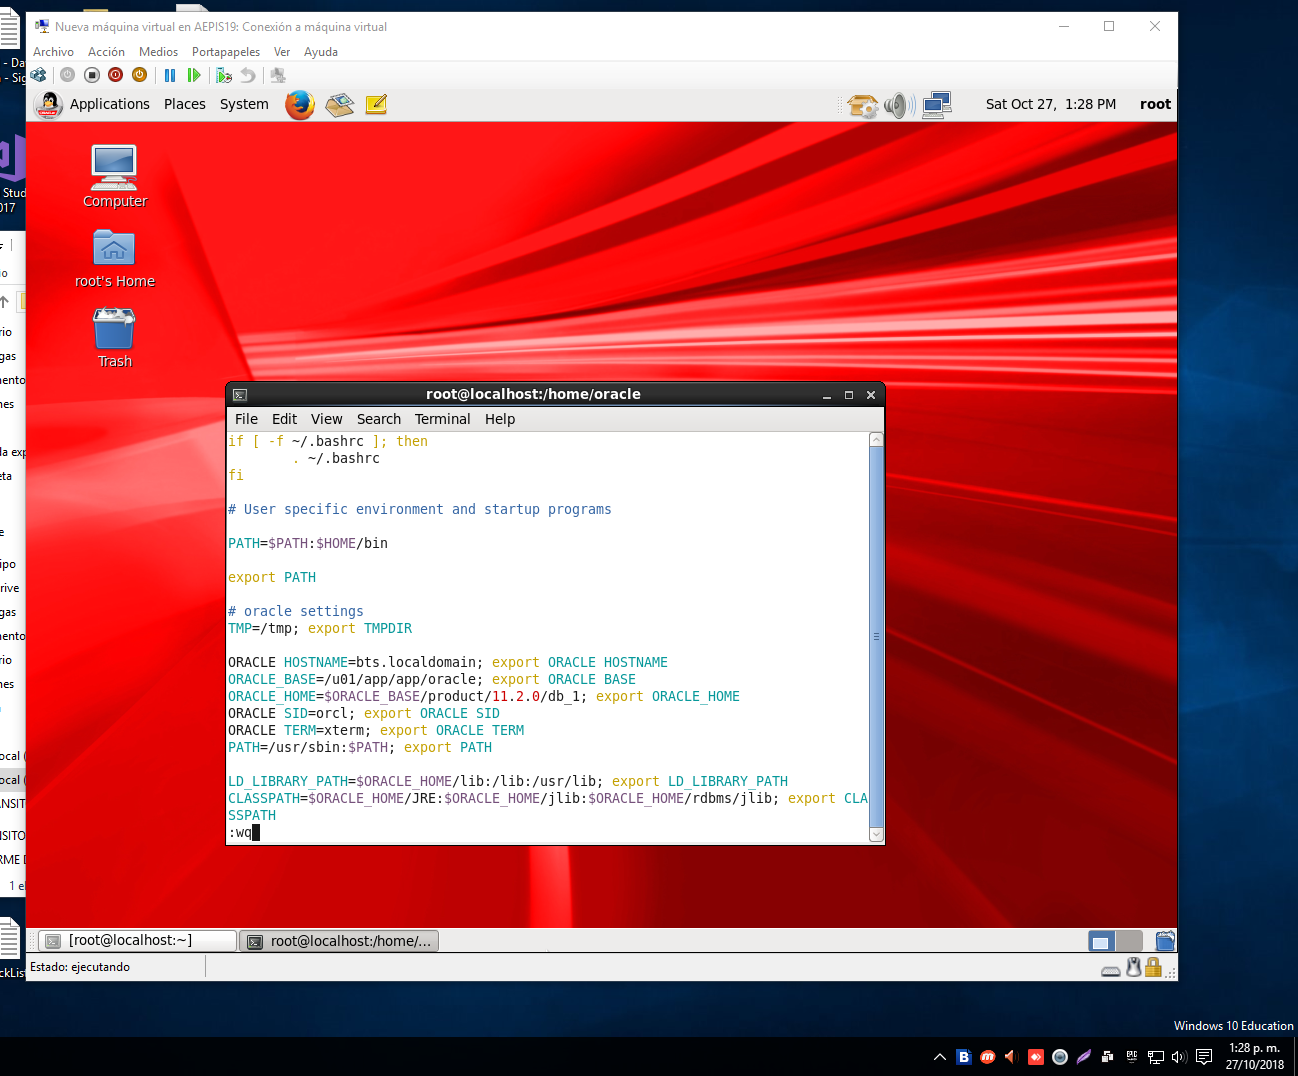
\includegraphics[width=13cm]{./Imagenes/imagen21} 
	\end{center}

\section{Paso 22:}
	\item En este paso vamos sistema de archivos. 
	\begin{center}
	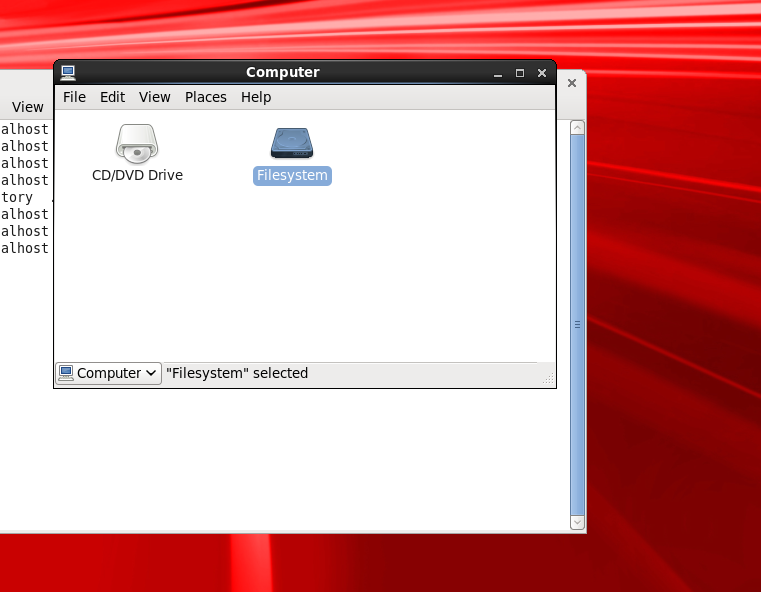
\includegraphics[width=13cm]{./Imagenes/imagen22} 
	\end{center}
	
	
\newpage
\section{Paso 23:}
	\item continuando con la instalacion del Oracle.
	\begin{center}
	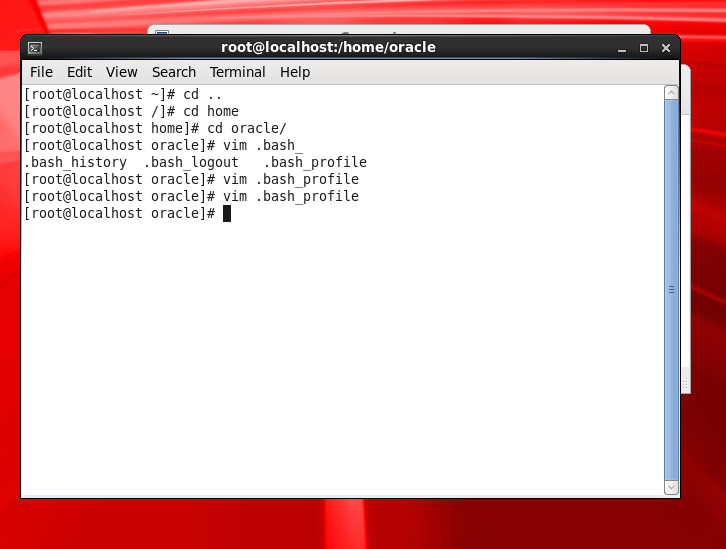
\includegraphics[width=13cm]{./Imagenes/imagen23} 
	\end{center}

\end{itemize} 
\end{document}

\begin{itemize}
\begin{center}
    Paso 24
\end{center}

    Seguidamente ingresamos al menu principal en modo grafico y hacemos clik en la opcion de Network Connections para poder realizar las configuraciones.
	\begin{center}
	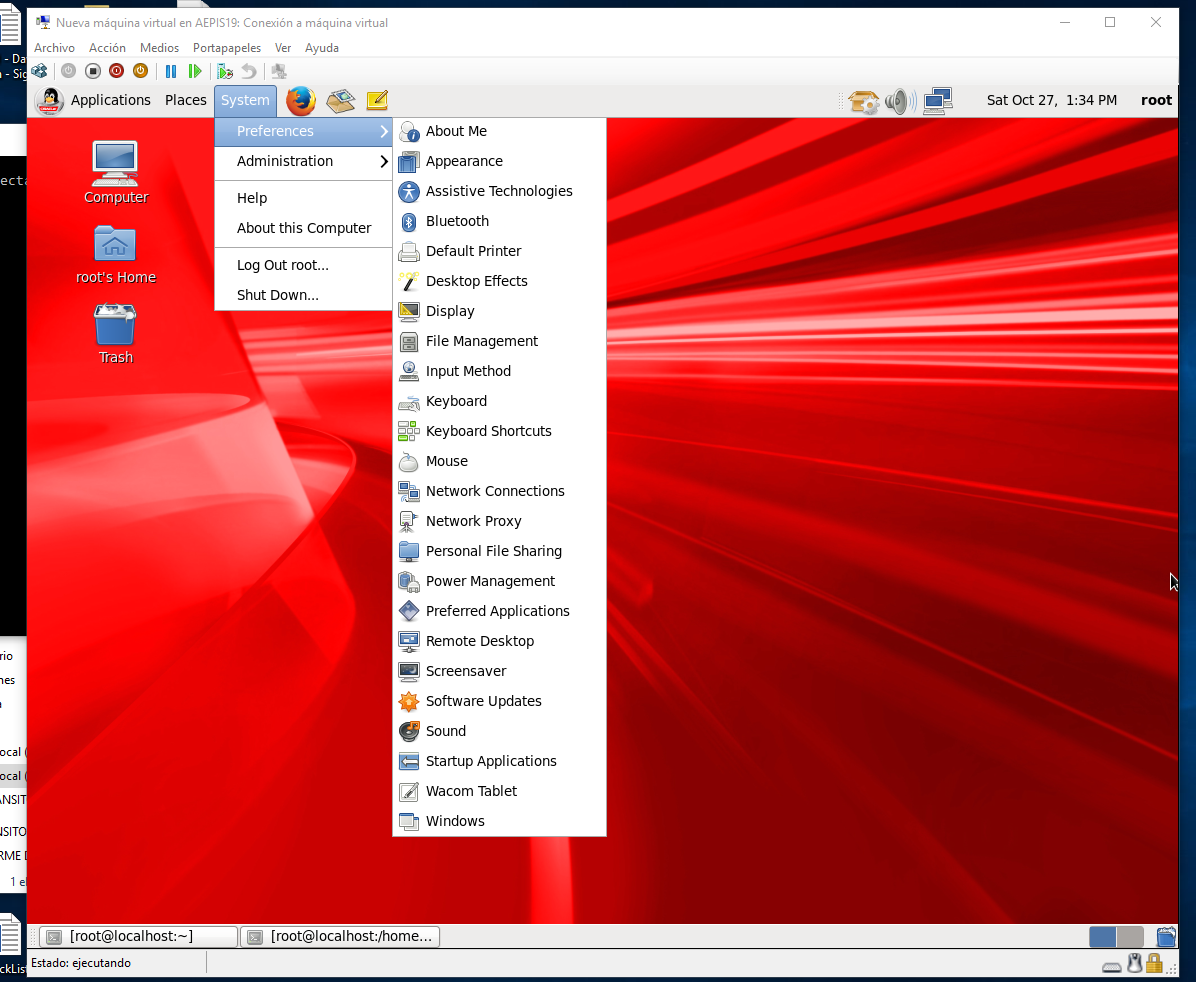
\includegraphics[width=15cm]{./Imagenes/imagen24} 
	\end{center}

\end{itemize} 

\begin{itemize}
\begin{center}
    Paso 25
\end{center}

    Luego nos muestra la ventana de de configuracion de IP. 
	\begin{center}
	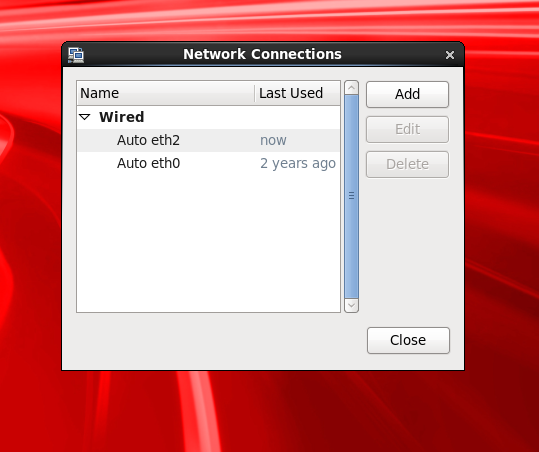
\includegraphics[width=15cm]{./Imagenes/imagen25} 
	\end{center}

\end{itemize} 

\begin{itemize}
\begin{center}
    Paso 26
\end{center}

    Seguidamente realizamos las asignaciones de IP de forma manual\\
	\begin{center}
	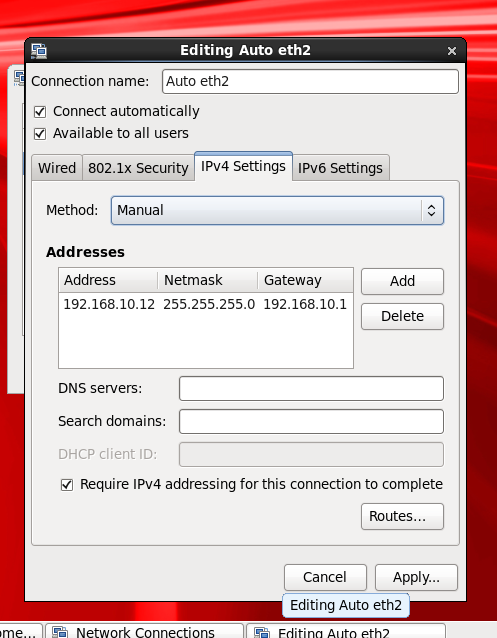
\includegraphics[width=15cm]{./Imagenes/imagen26} 
	\end{center}

\end{itemize} 

\begin{itemize}
\begin{center}
    Paso 27
\end{center}

    Luego agregamos la configuracion y aceptamos\\
	\begin{center}
	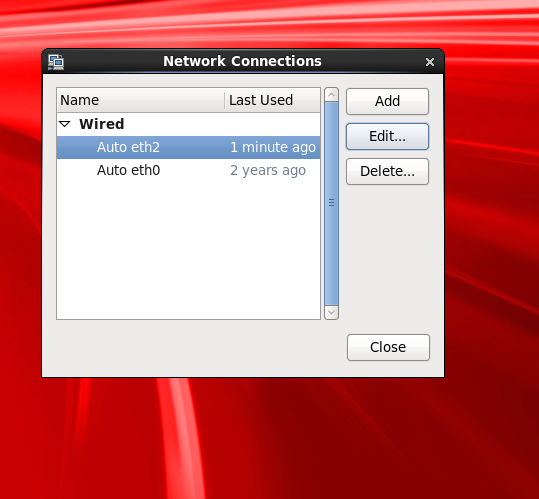
\includegraphics[width=15cm]{./Imagenes/imagen27} 
	\end{center}

\end{itemize} 

\begin{itemize}
\begin{center}
    Paso 28
\end{center}

    Nos dirigimos a Windows y abrimos el cmd para poder consultar el IP para lo cual utilizamos el ipconfig que nos muestra solo los datos esenciales como la Dirección IP, la Máscara de red y la Puerta de enlace, para cada adaptador encontrado.\\
	\begin{center}
	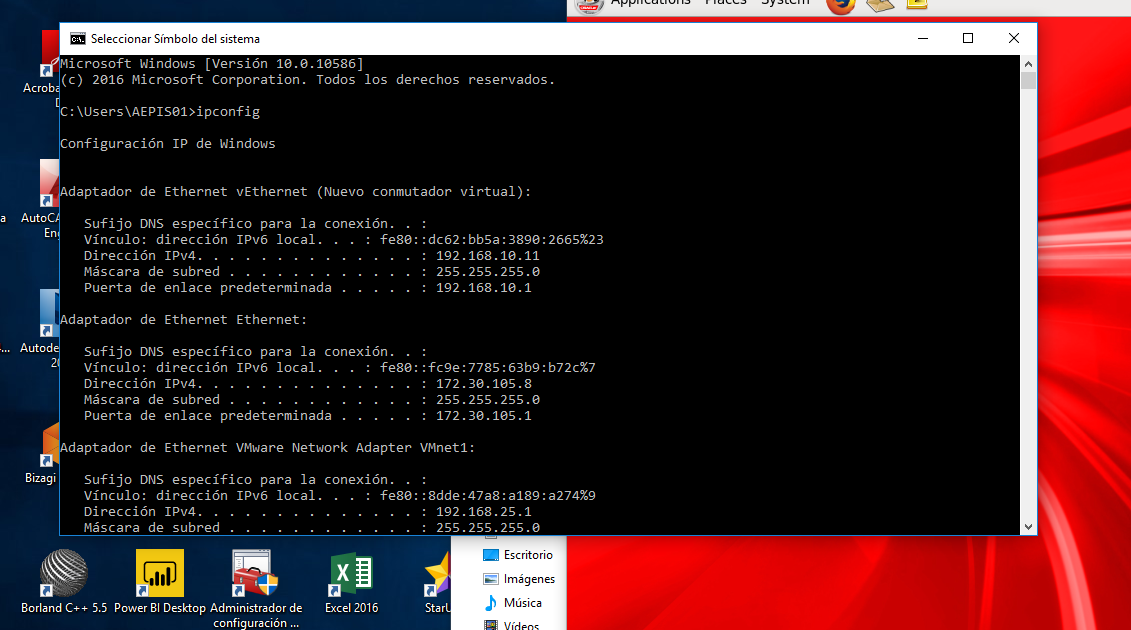
\includegraphics[width=15cm]{./Imagenes/imagen28} 
	\end{center}

\end{itemize} 

\begin{itemize}
\begin{center}
    Paso 29
\end{center}

    Realizamos el ping que es un comando o una herramienta de diagnóstico que permite hacer una verificación del estado de una determinada conexión de un host local con al menos un equipo remoto contemplado en una red de tipo TCP/IP \\
	\begin{center}
	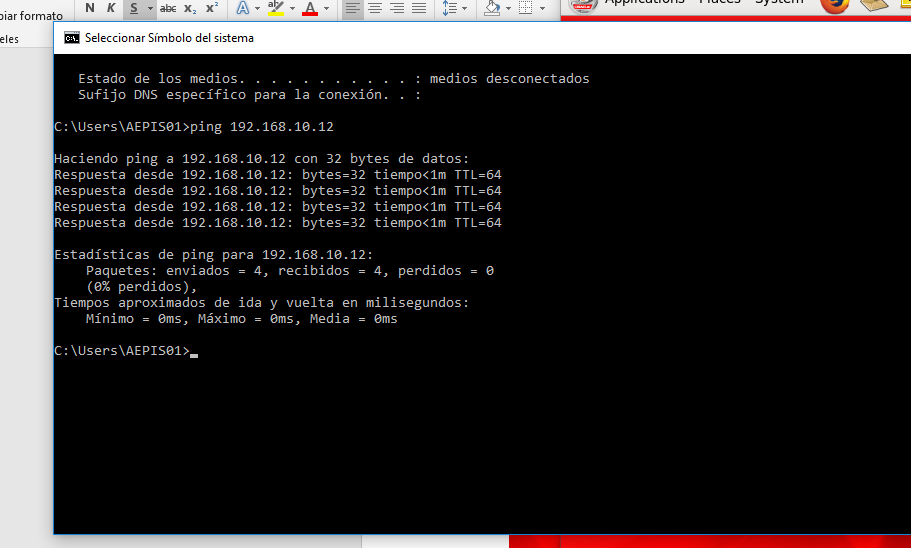
\includegraphics[width=15cm]{./Imagenes/imagen29} 
	\end{center}

\end{itemize} 

\begin{itemize}
\begin{center}
    Paso 30
\end{center}

    Seguidamente nos dirigimos a nuestra maquina virtual e ingresamos al directorio home \\
	\begin{center}
	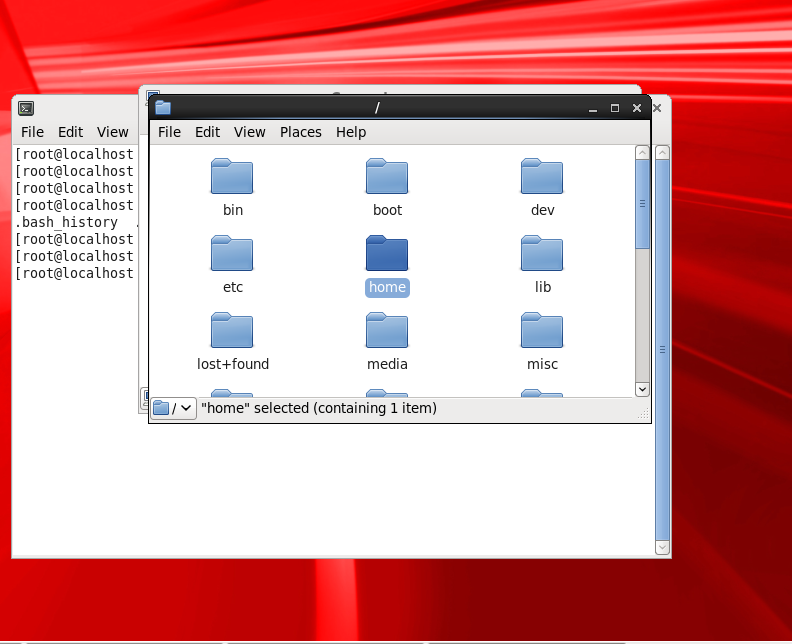
\includegraphics[width=15cm]{./Imagenes/imagen30} 
	\end{center}

\end{itemize} 

\begin{itemize}
\begin{center}
    Paso 31
\end{center}

    Desconprimimos los 2 archivos que se encuentran\\
	\begin{center}
	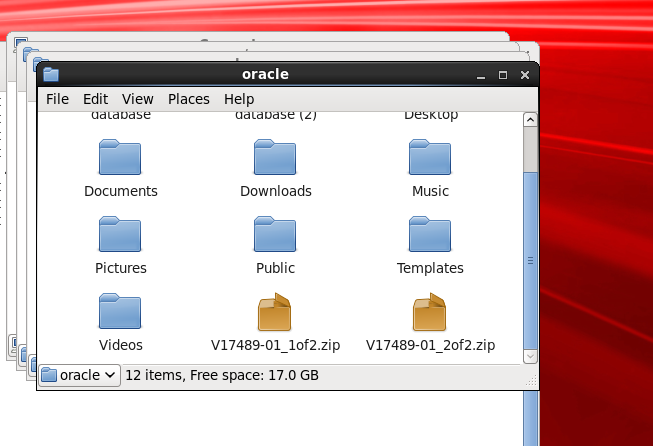
\includegraphics[width=15cm]{./Imagenes/imagen31} 
	\end{center}

\end{itemize} 


\begin{itemize}
\begin{center}
    Paso 32
\end{center}

    Una vez descomprimido ejecutamos el archivo\\
	\begin{center}
	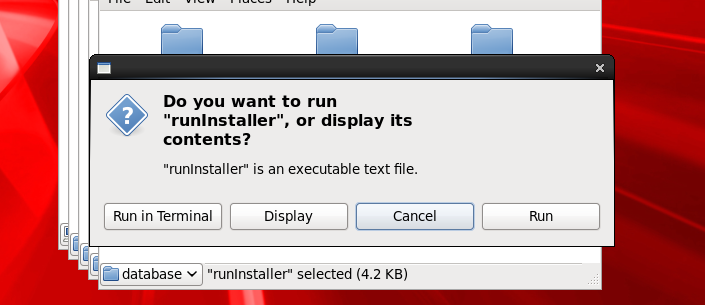
\includegraphics[width=15cm]{./Imagenes/imagen32} 
	\end{center}

\end{itemize} 


\section{Instalacion base de datos Oracle} 
\begin{itemize}
	\item Una vez iniciada la sesión con el usuario “oracle”, abrir una ventana de Terminal y editar el archivo
bashprofile,Escribimos las siguientes lineas dentro del archivo bashprofile.
	\begin{center}
	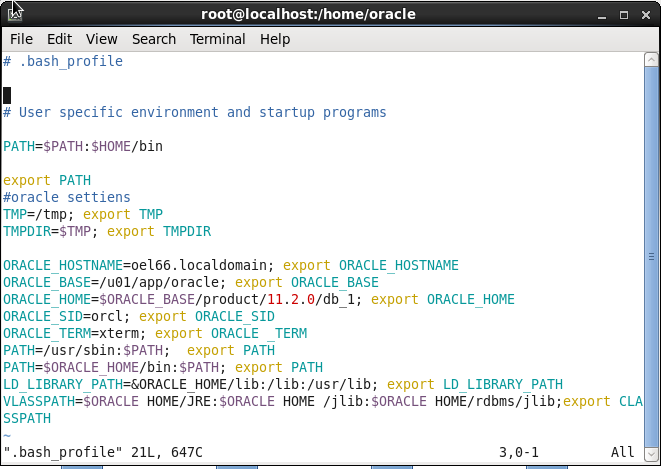
\includegraphics[width=14cm]{./Imagenes/img44} 
	\end{center}
	
	\item Ahora descomprimimos el archivo VT7489-01lof2.zip y el archivo VT7489-01lof2.zip . el cual creara una carpeta database como se muestra en la imagen
	\begin{center}
	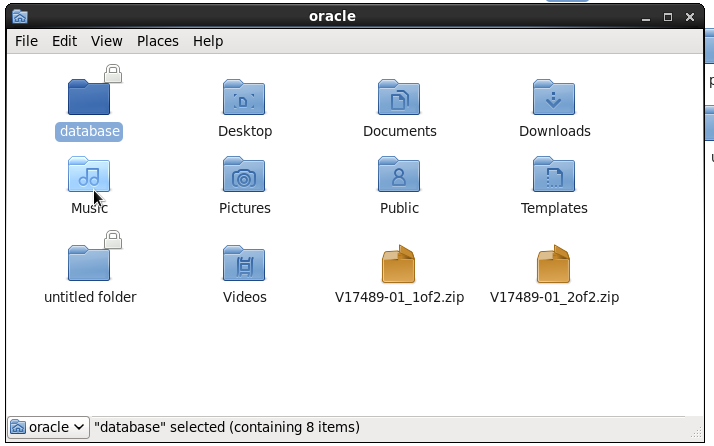
\includegraphics[width=14cm]{./Imagenes/img45} 
	\end{center}
\newpage
	\item Ahora iniciamos la instlacion de la base de datos Oracle haciendo doble clic sobre el archivo bash de instalacion y nos mostrara la siguiente venta presionamos en run, y saldra el menu de instalacion de de oracle.
	\begin{center}
	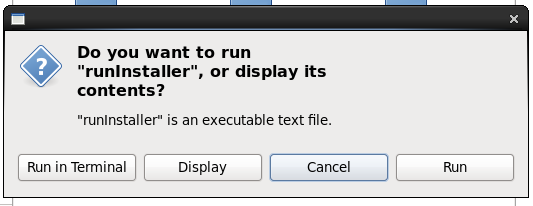
\includegraphics[width=14cm]{./Imagenes/img47} 
	\end{center}
	
	\item El menu de instalacion de oracle se mostrara como enla imagen en el cual escribiremos cualquier correo desmarcaremos el chek y presionaremos en siguiente para continuar la instalacion de la base de datos oracle.
	\begin{center}
	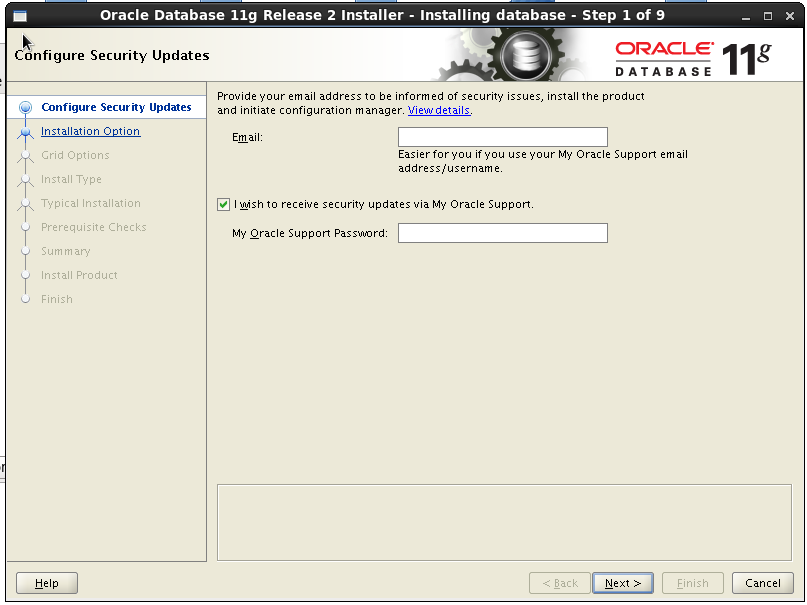
\includegraphics[width=14cm]{./Imagenes/img48} 
	\end{center}
\newpage

	\item Nos mostrara los siguientes de datos de instalcion elcual marcaremos el radiobutton de la opcion de crear y configurar una base de datos y presionaremos en siguiente.
	\begin{center}
	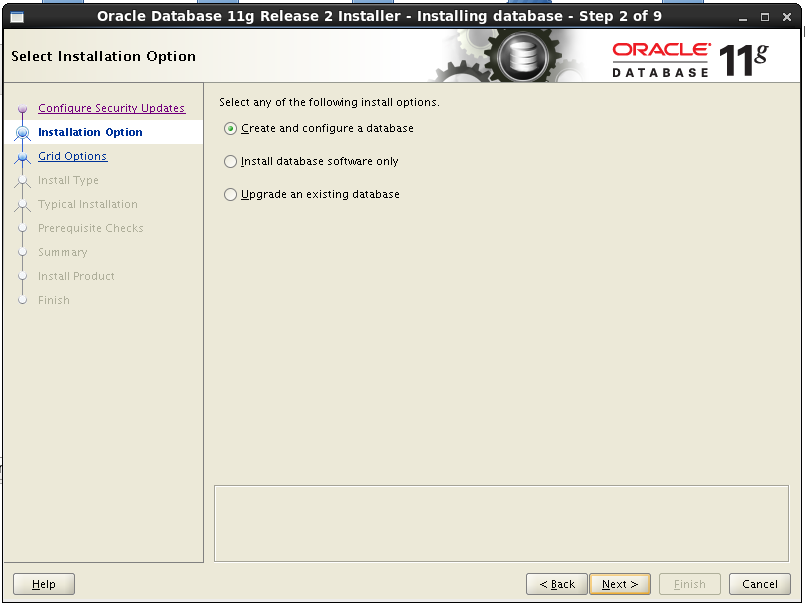
\includegraphics[width=13cm]{./Imagenes/img49} 
	\end{center}
	
	\item En este paso marcamos la opcion de server Class y preisonamos el boton de siguiente.
	\begin{center}
	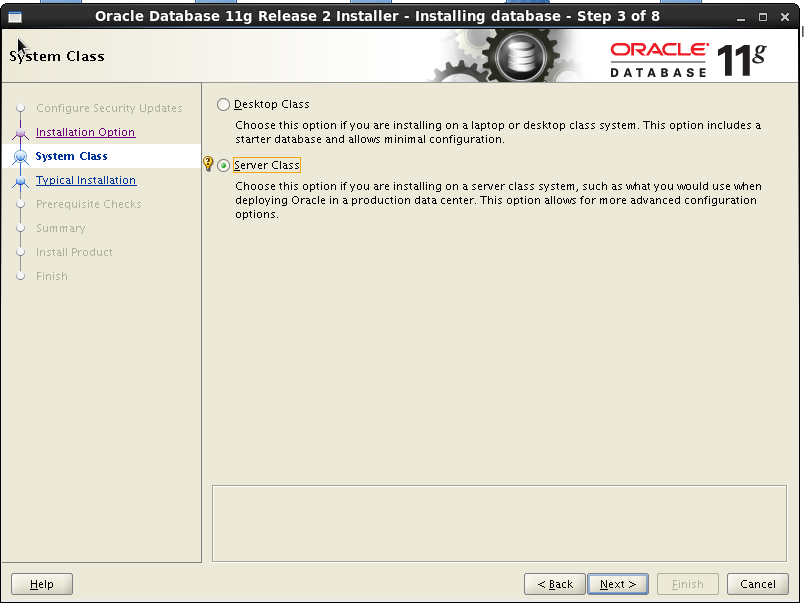
\includegraphics[width=13cm]{./Imagenes/img50} 
	\end{center}
	
\newpage

	\item Dejamos marcado la opcion por defecto y presionamos en el boton de siguiente para continuar con la instalacion de la base de datos oracle .
	\begin{center}
	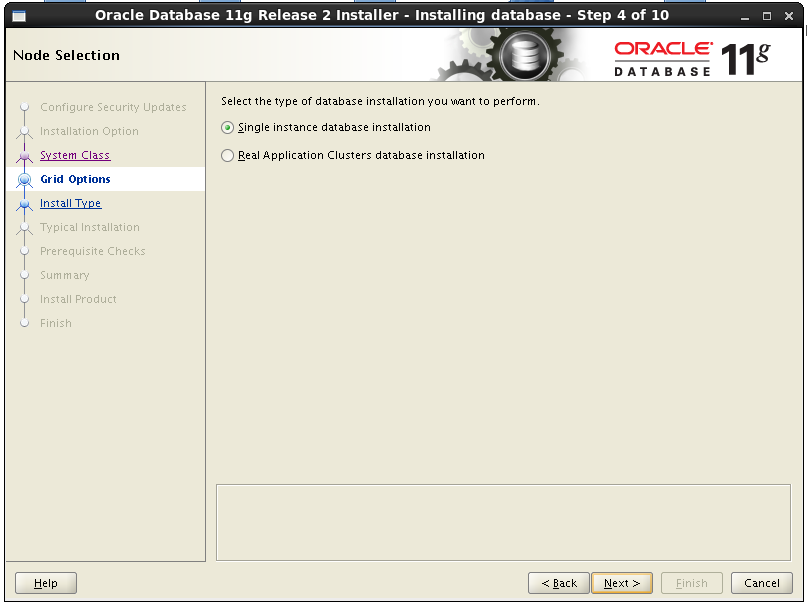
\includegraphics[width=13cm]{./Imagenes/img51} 
	\end{center}
	
	\item En este paso dejamos marcado la opcion de instalcion tipica y luego preisonamos la opcion de continuar.
	\begin{center}
	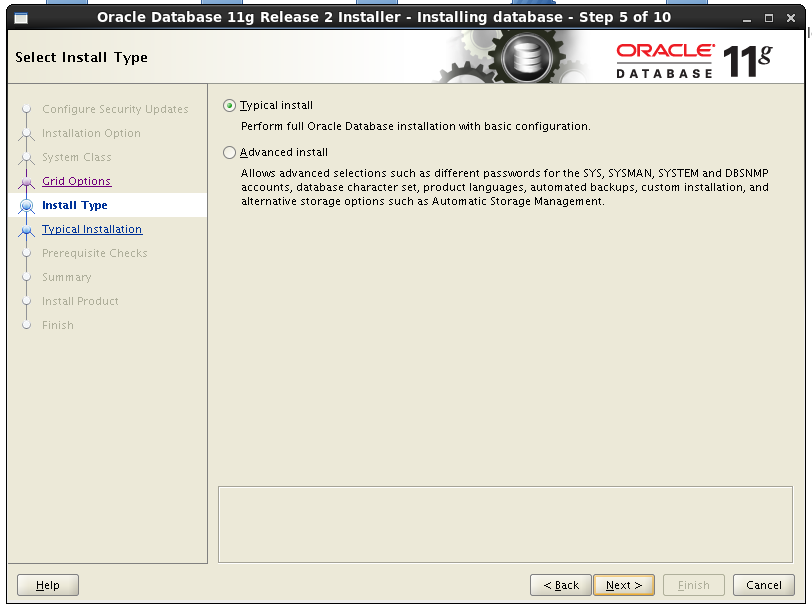
\includegraphics[width=13cm]{./Imagenes/img52} 
	\end{center}
	
	
\newpage

	\item Nos aparece la siguiente ventana el cual vamos a omitir este marcando la opcion de ignorar todo que se encuentra en la esquina superior derecha y el boton de siguiente se activara.
	\begin{center}
	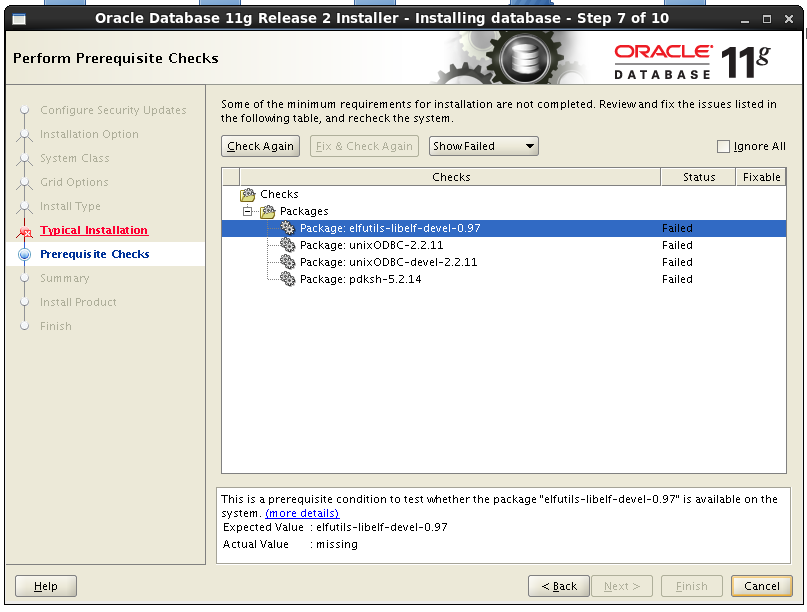
\includegraphics[width=13cm]{./Imagenes/img53} 
	\end{center}
	
	\item Nos mostrara un resumen de todas las opciones que emos selccionado .
	\begin{center}
	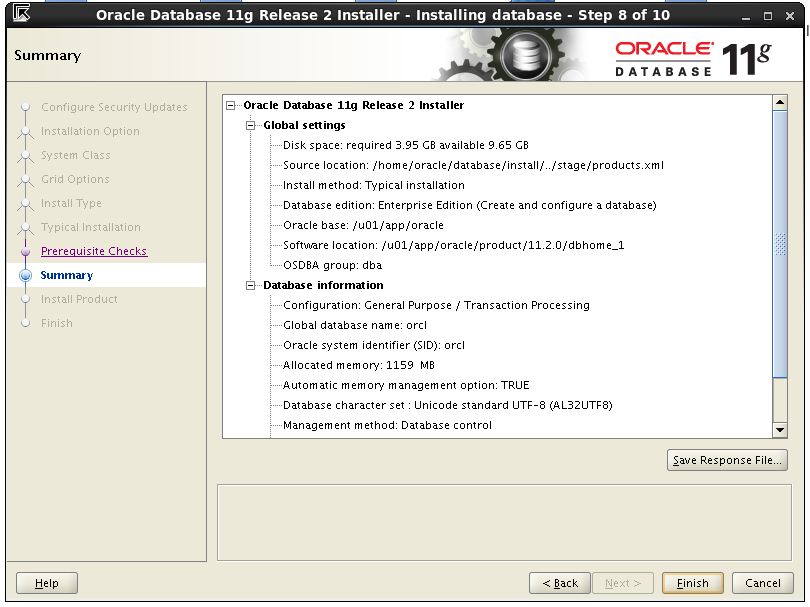
\includegraphics[width=13cm]{./Imagenes/img54} 
	\end{center}
	
	
\newpage

	\item Esperamos que la instalacion termine ,nos mostrara un cuadro donde nos muestra el estado de instalacion.
	\begin{center}
	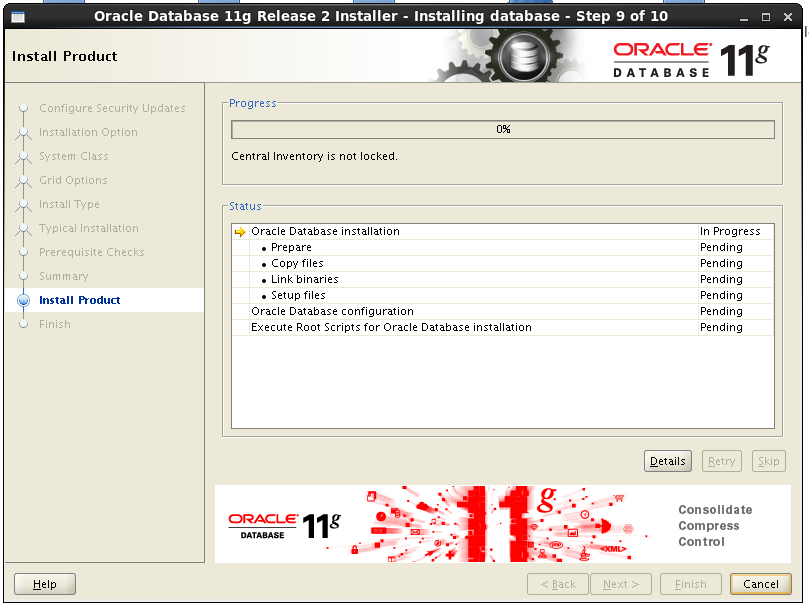
\includegraphics[width=13cm]{./Imagenes/img55} 
	\end{center}
	
	\item En este paso vamos a llenar los datos necesarios que nos pidepara continuar con la instalacion .
	\begin{center}
	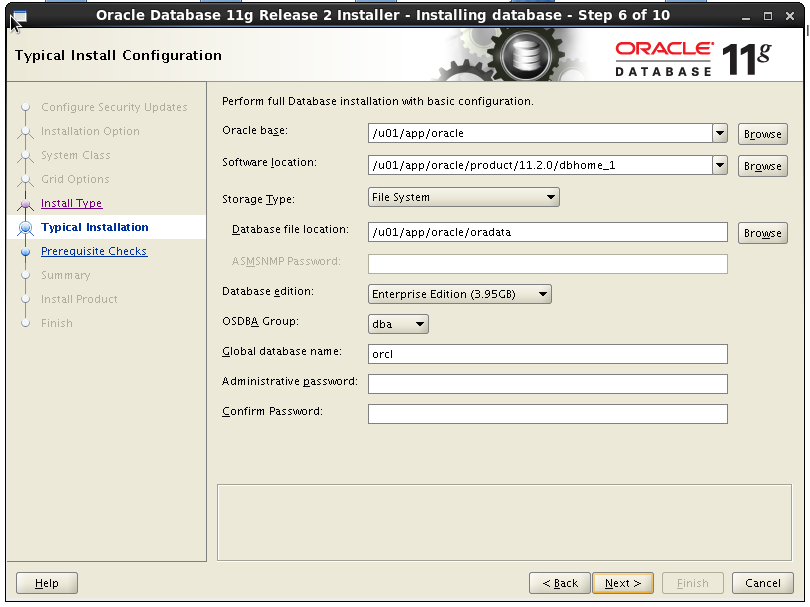
\includegraphics[width=13cm]{./Imagenes/img56} 
	\end{center}
	
	
\newpage

	\item Cuando estemos instalando la base de datos nos mostrara un mensaje que nos dice que se esta copiando la base de datos.
	\begin{center}
	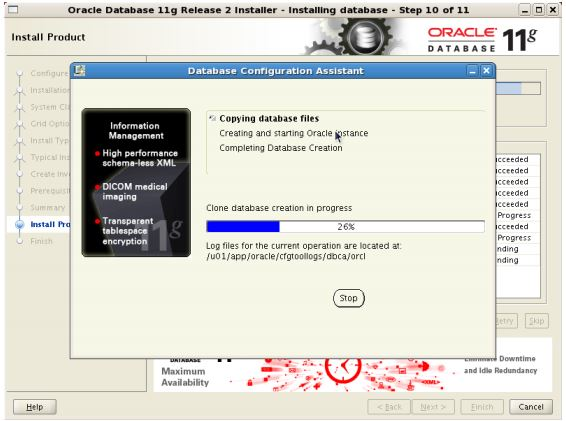
\includegraphics[width=13cm]{./Imagenes/img57} 
	\end{center}
	
	\item Al terminar la instalcion nos mostrara este mensaje donde nos muestra la informacionde la instalacion .
	\begin{center}
	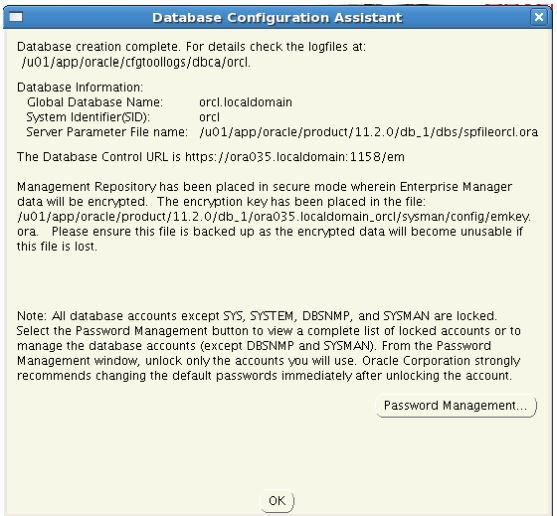
\includegraphics[width=10cm]{./Imagenes/img58} 
	\end{center}
	
	
\newpage

	\item Nos mostrara una ventana ,ahora cambiamos de usuario a usuario root y copiamos las dos rutas mostras a continuacion y pegaos en una terminal al final presionamos exit.
	\begin{center}
	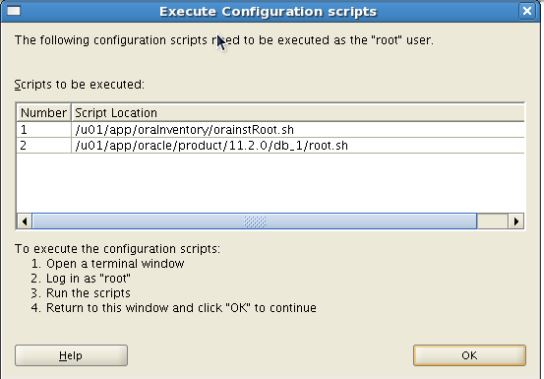
\includegraphics[width=13cm]{./Imagenes/img59} 
	\end{center}
	
	\item Nos saldra el mensaje de fin de la instalacion presionamos en exit   .
	\begin{center}
	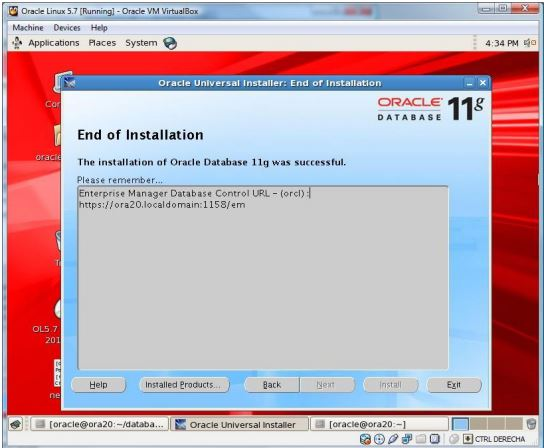
\includegraphics[width=10cm]{./Imagenes/img60} 
	\end{center}
	
\newpage

	\item Ahora tendremos que abrir un navegador y poner la siguiente direccion para que nos redireccione al gestor de base de datos de oracle.
	\begin{center}
	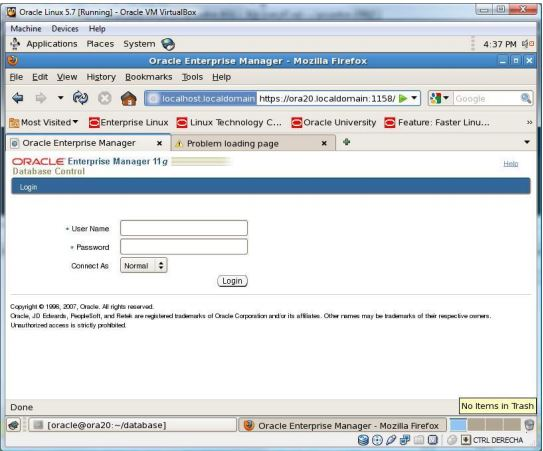
\includegraphics[width=13cm]{./Imagenes/img61} 
	\end{center}



\end{itemize} 
\newpage

\section{Cuestionario} 
	\item Los valores introducidos al archivo sysctl.conf ¿que representan?\\.
	fs.suiddumpable\\
    fs.aio-max-nr\\
    fs.file-max\\
    kernel.shmmni\\
    kernel.sem\\
    net.ipv4.iplocalortrange\\
    net.core.rmemdefault\\
    net.core.rmemmax\\
    net.core.wmemdefault\\
    net.core.wmemmax\\
   \item ¿Con qué usuario(s) puedo conectarme al servidor a través del AdministradorEmpresarial?\\
   Con el usuario SYS

\include{Secciones/bibliografia}


\end{document}
